% !TeX root = ../../../main.tex

\begin{figure}
	\centering
	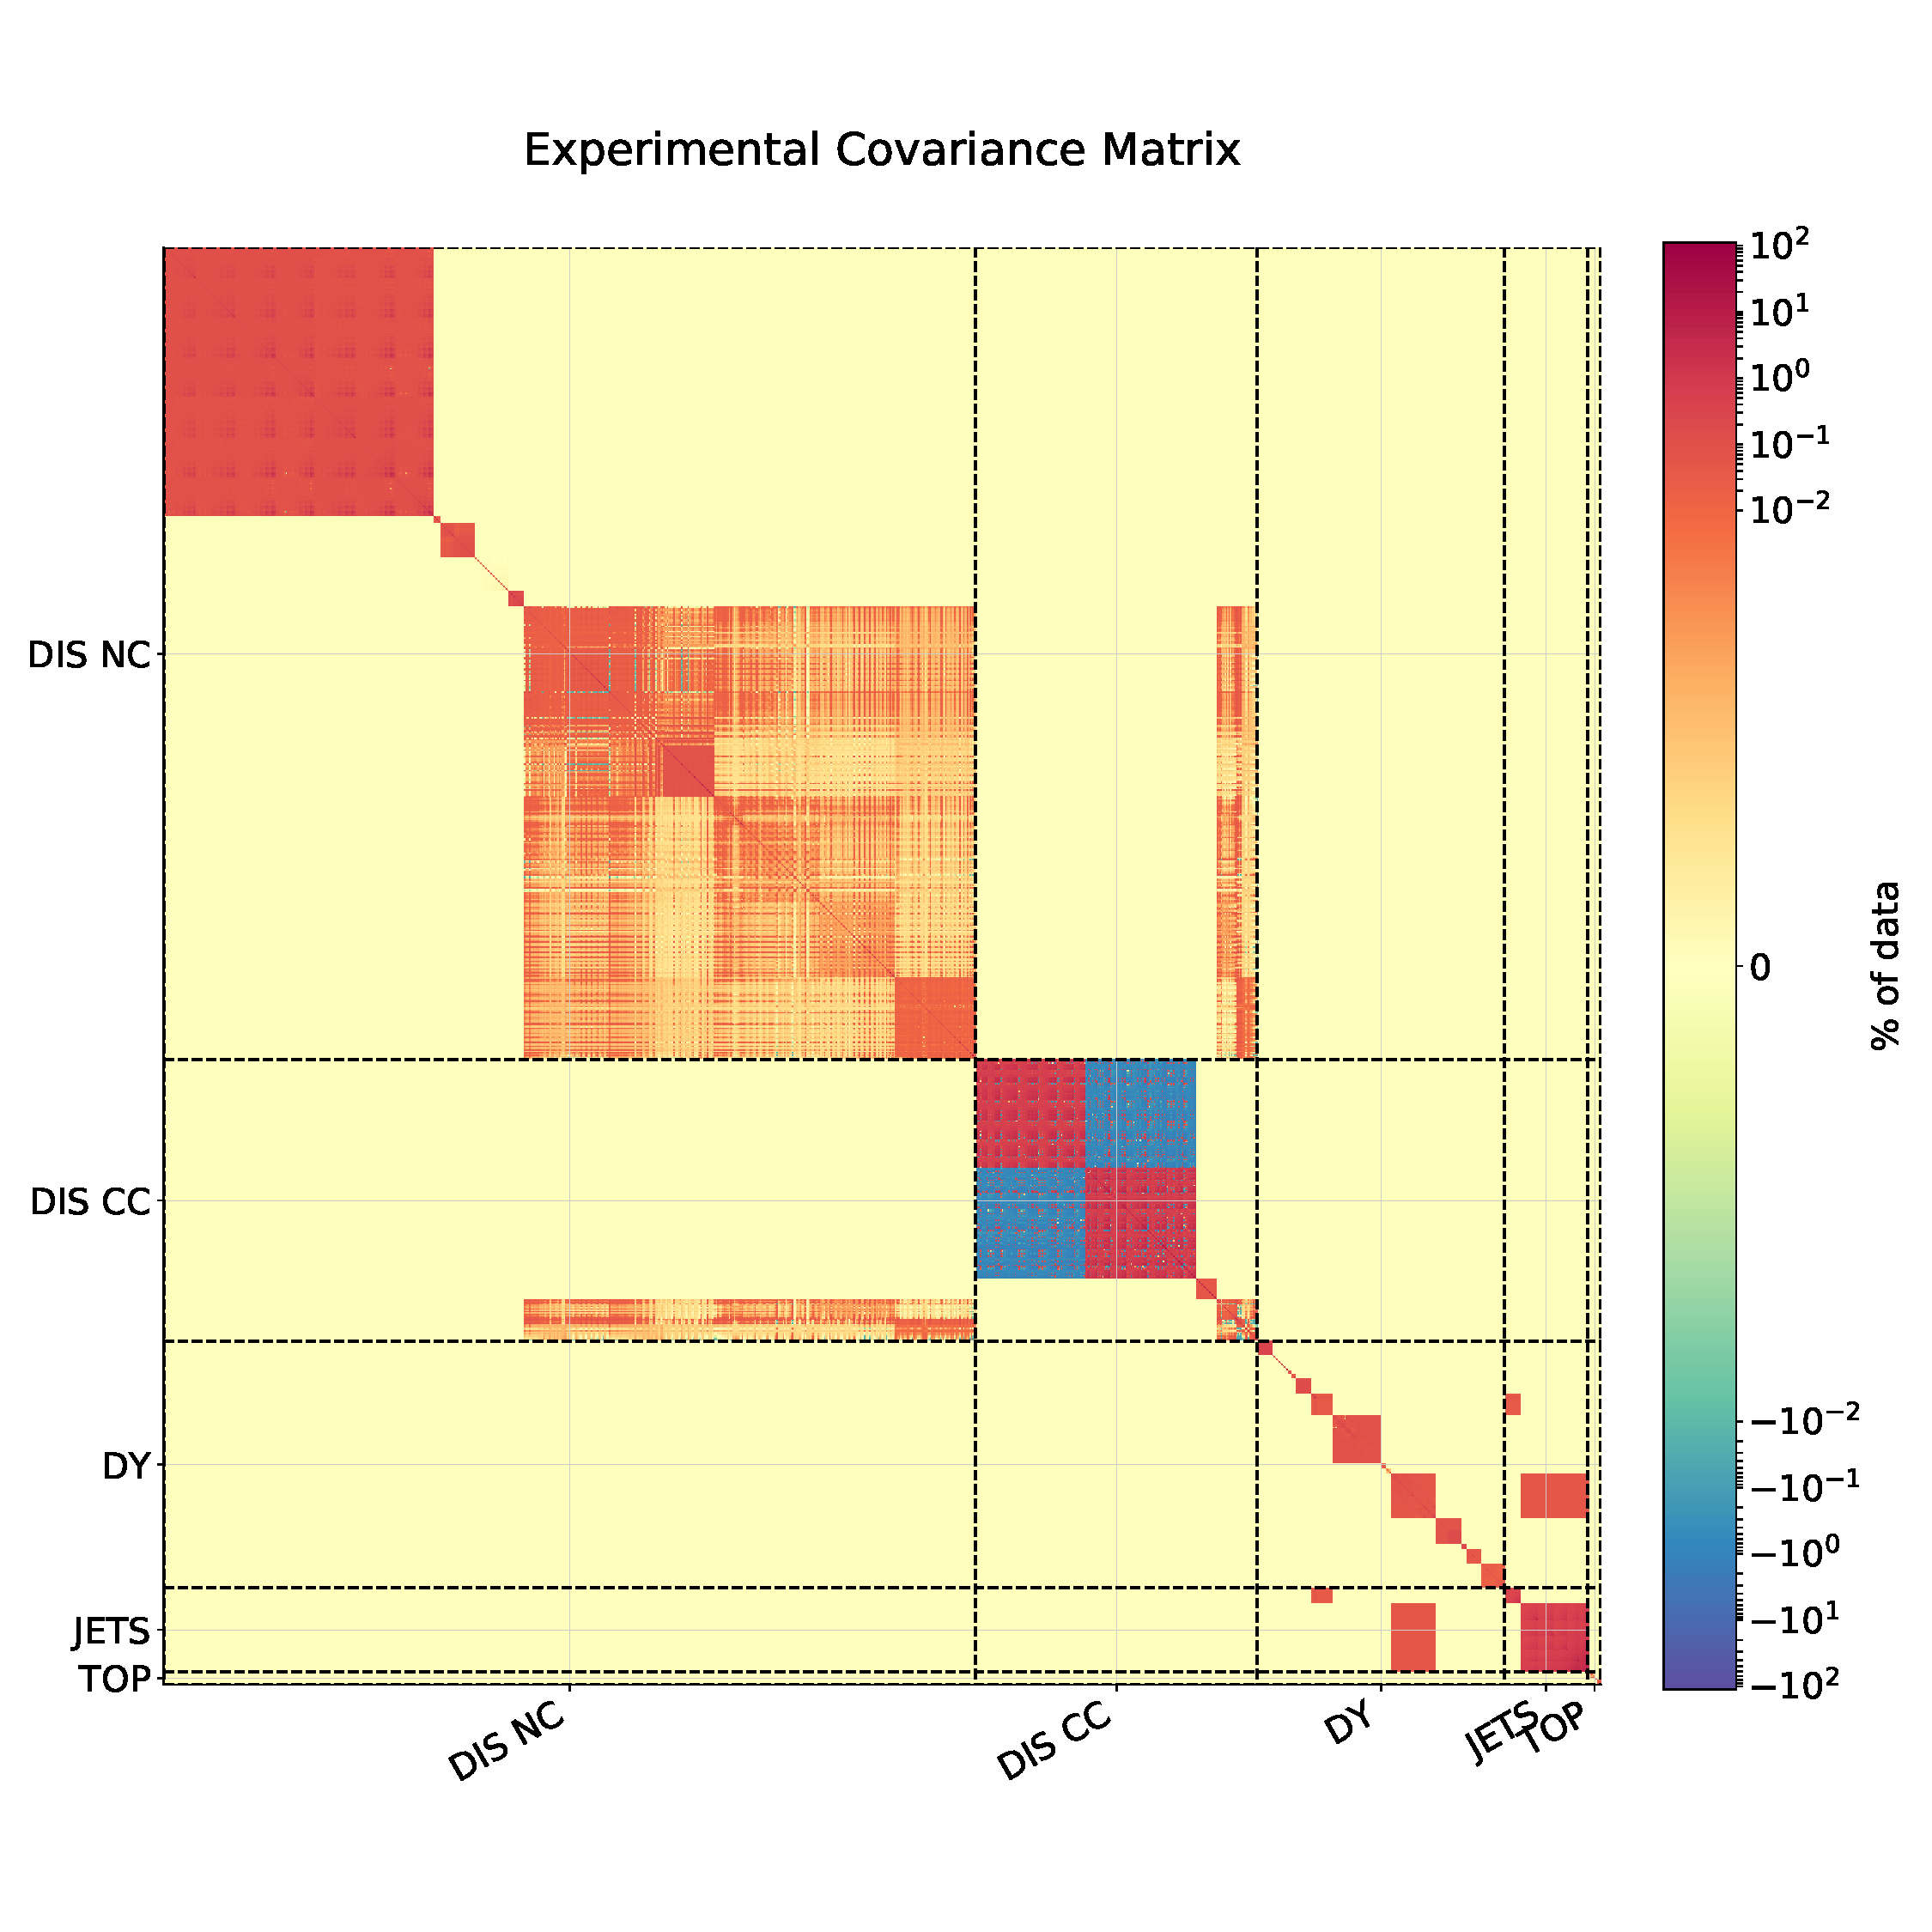
\includegraphics[width=0.49\hsize]{ch-mhou/exp_covmat}
	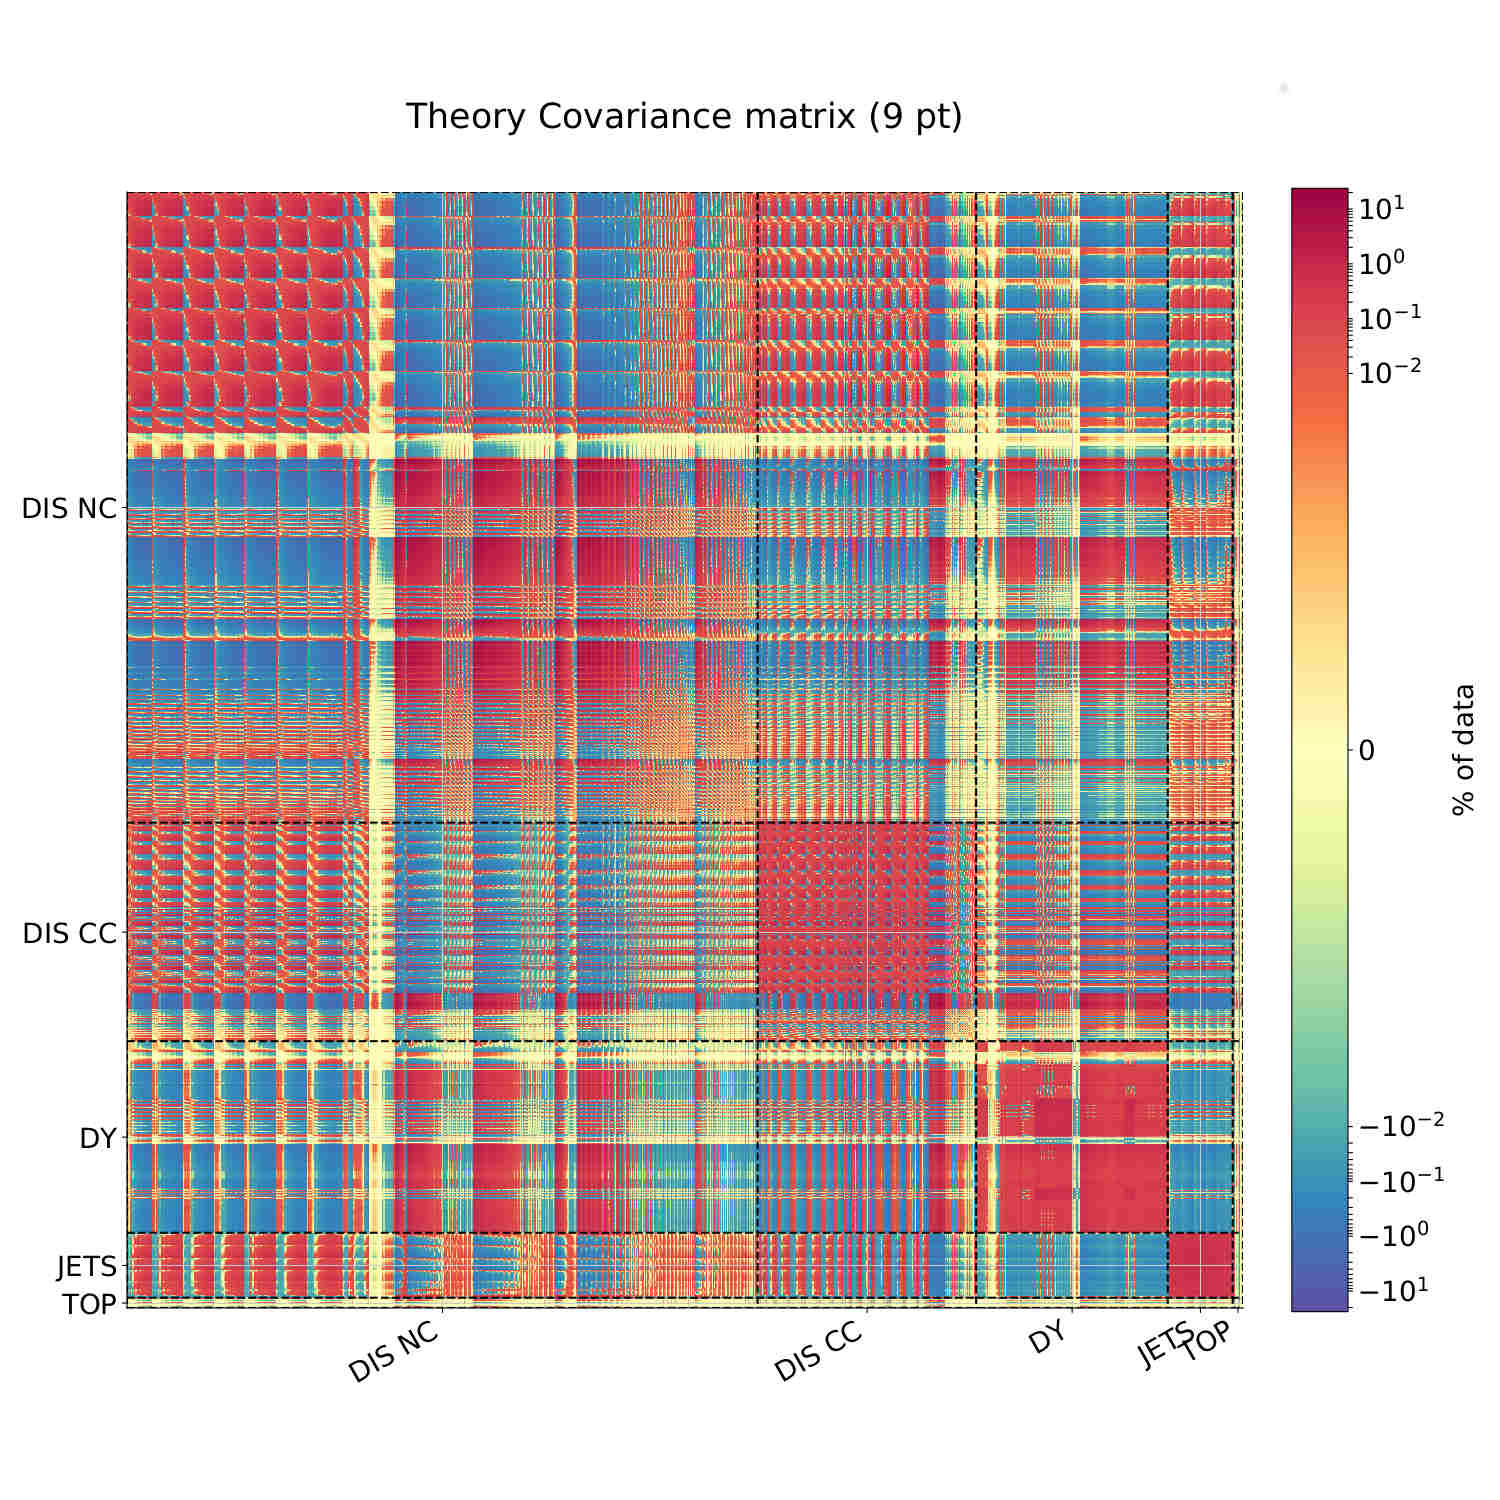
\includegraphics[width=0.49\hsize]{ch-mhou/th_covmat_9pt}
	\caption{
		Comparison between the experimental covariance matrix and the
		theoretical one, generated by the 9 point prescriptions, both
		normalized to central values.
	}
	\label{fig:pine/covmats}
\end{figure}

\begin{figure}
	\centering
	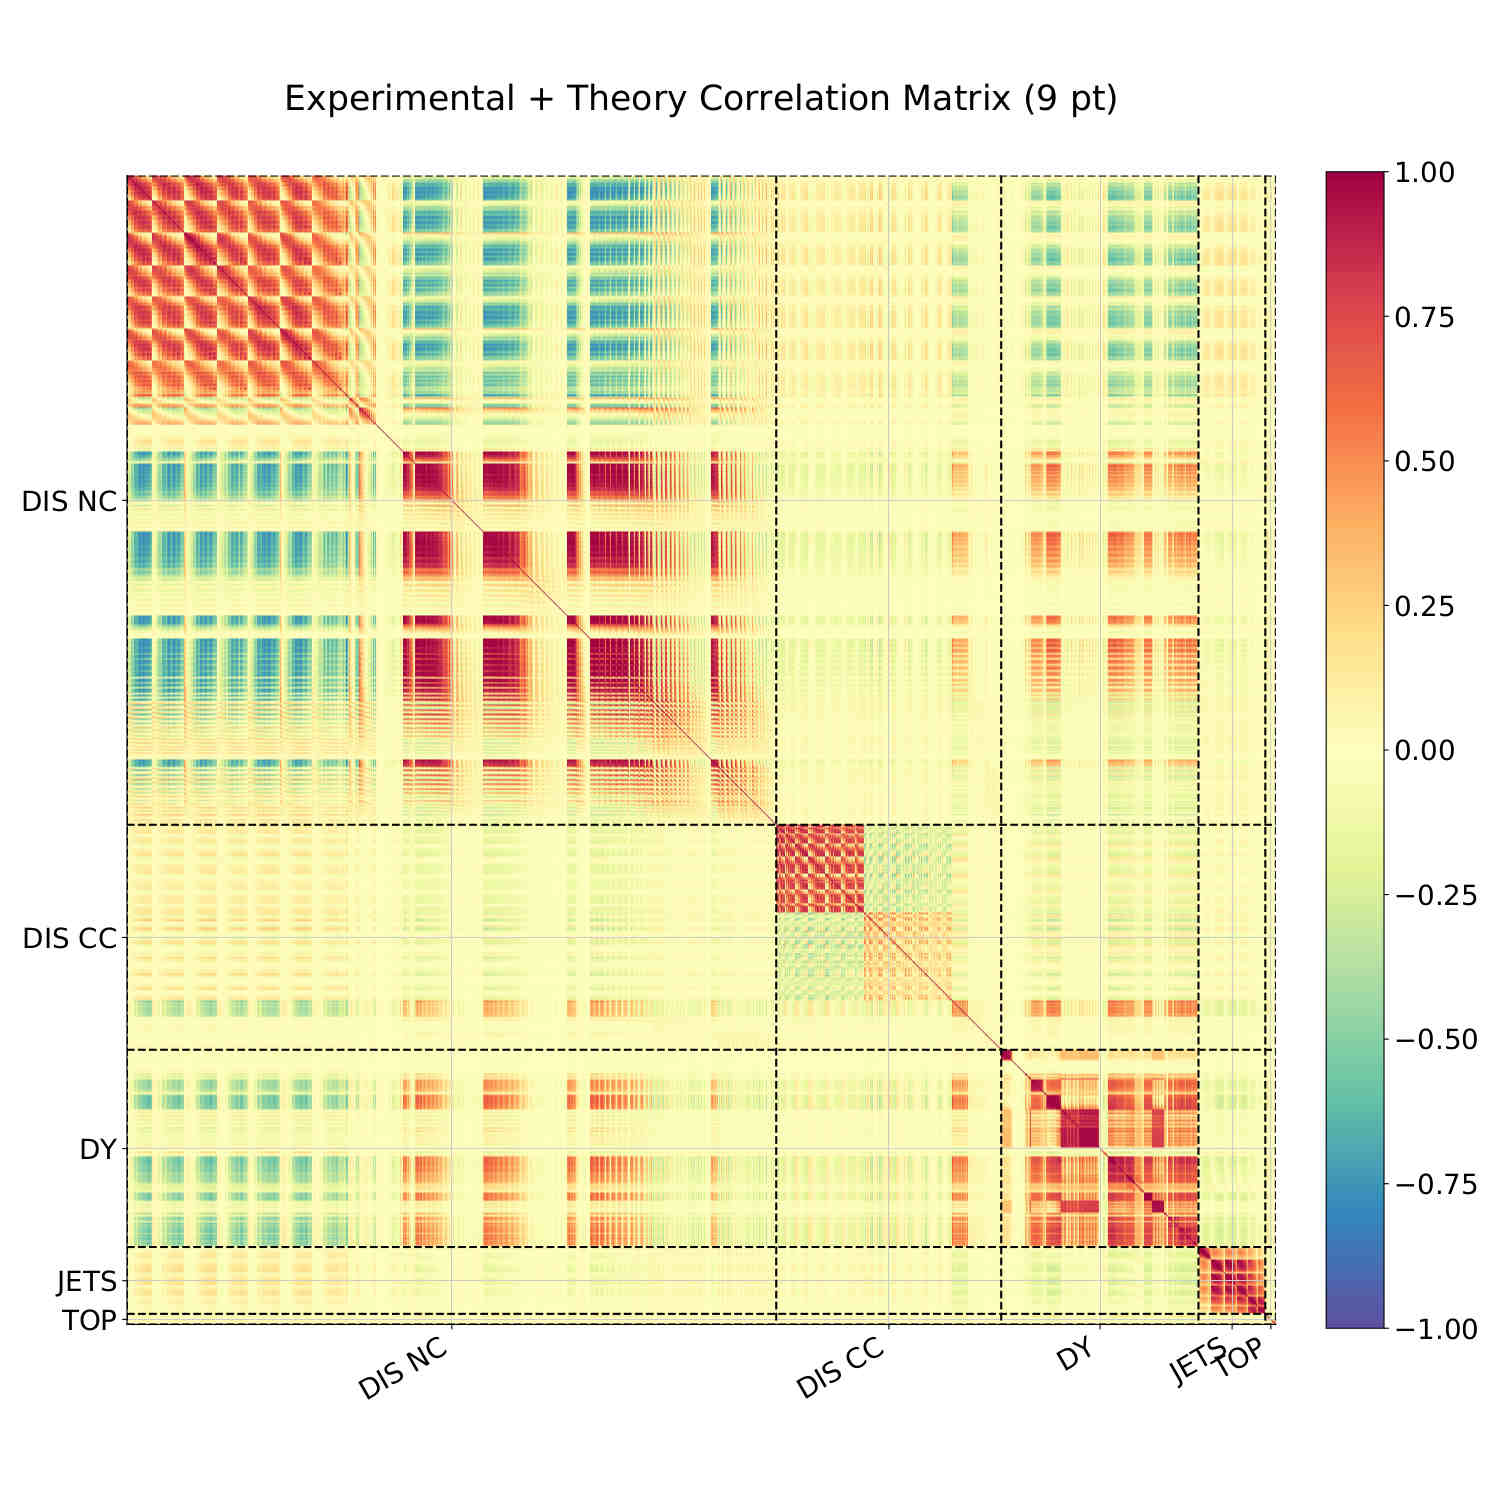
\includegraphics[width=0.7\hsize]{ch-mhou/expth_corrmat_9pt}
	\caption{
		Combined covariance matrix (experimental plus theoretical), the actual
		one used in the \nnpdfr[3.1th+]{3.1th} fit.
	}
	\label{fig:pine/combined-covmat}
\end{figure}

\begin{figure}
	\centering
	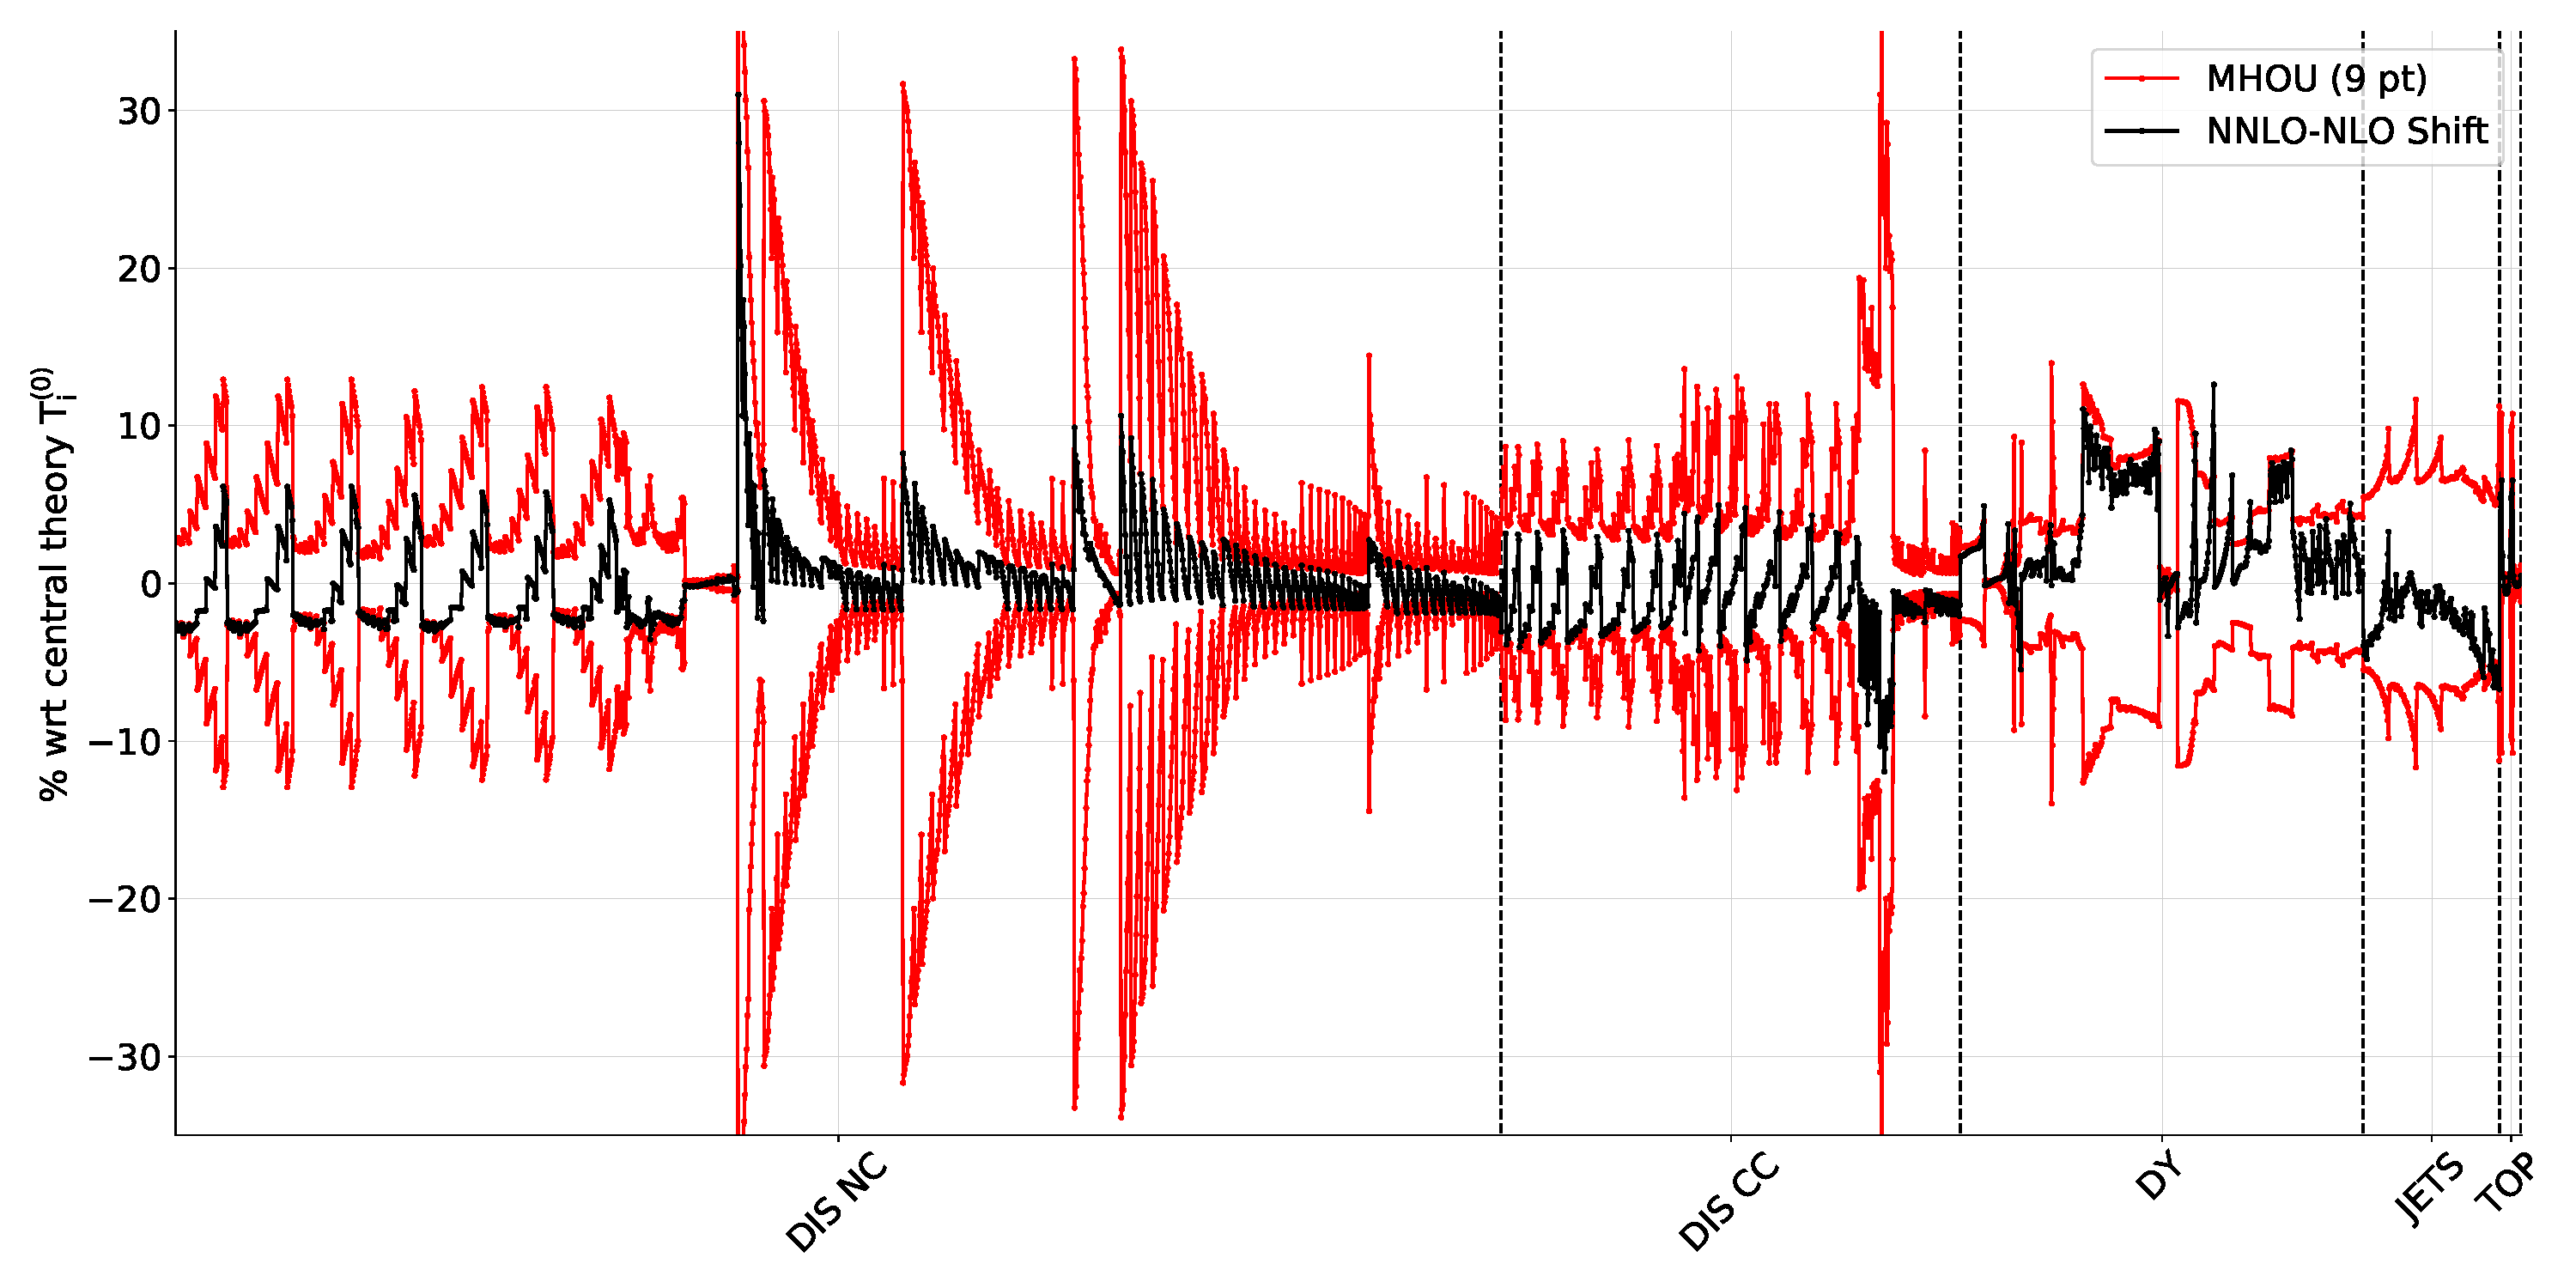
\includegraphics[width=\hsize]{ch-mhou/shift_diag_cov_comparison_9pt_global}
	\caption{
		The diagonal uncertainties $\sigma_i$ (red) symmetrized about zero,
		compared to the shift $\delta_i$ for each data-point (black).
		Values are shown as percentage of the central theory prediction
	}
	\label{fig:pine/scvar-shifts}
\end{figure}

\begin{figure}
	\centering
	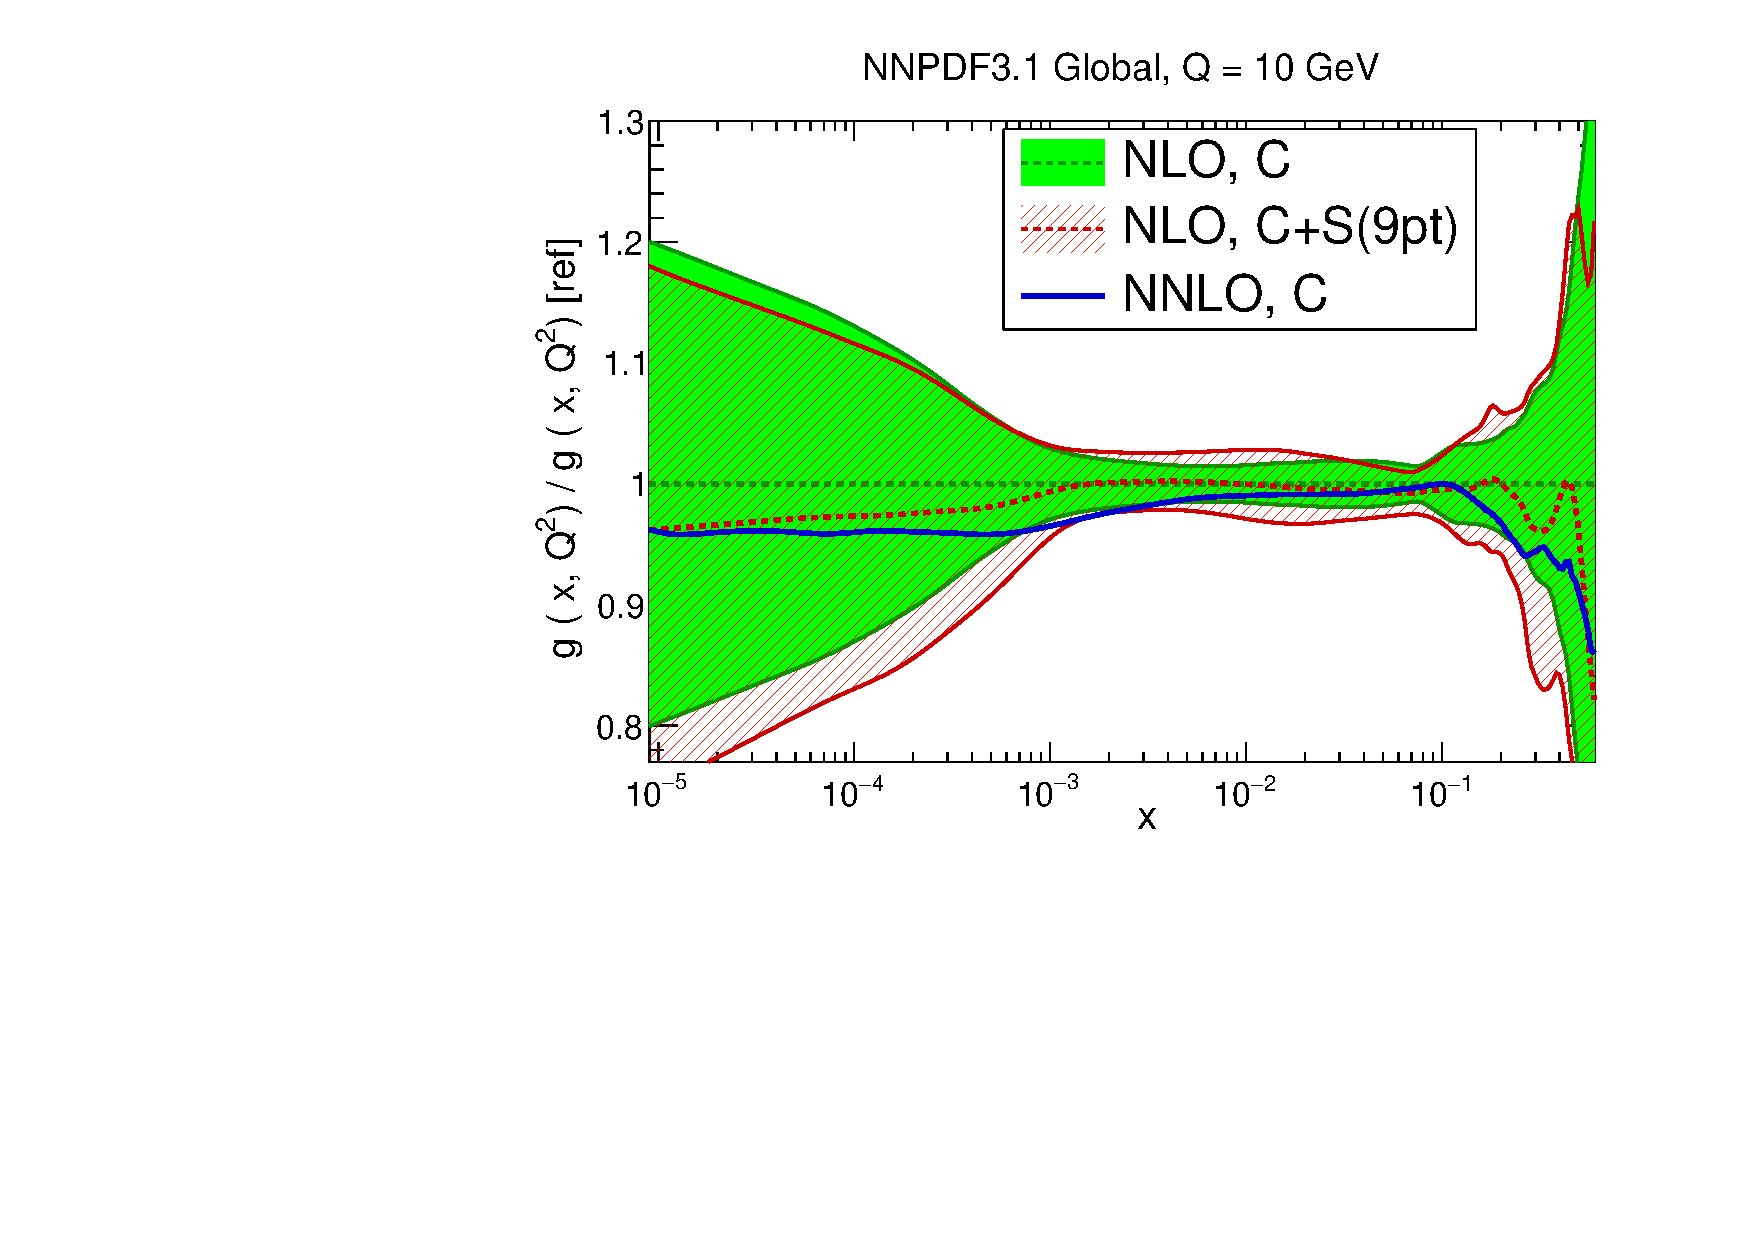
\includegraphics[width=0.49\hsize]{ch-mhou/xg-Global-NLO-CovMatTH-EXP-vsTH}
	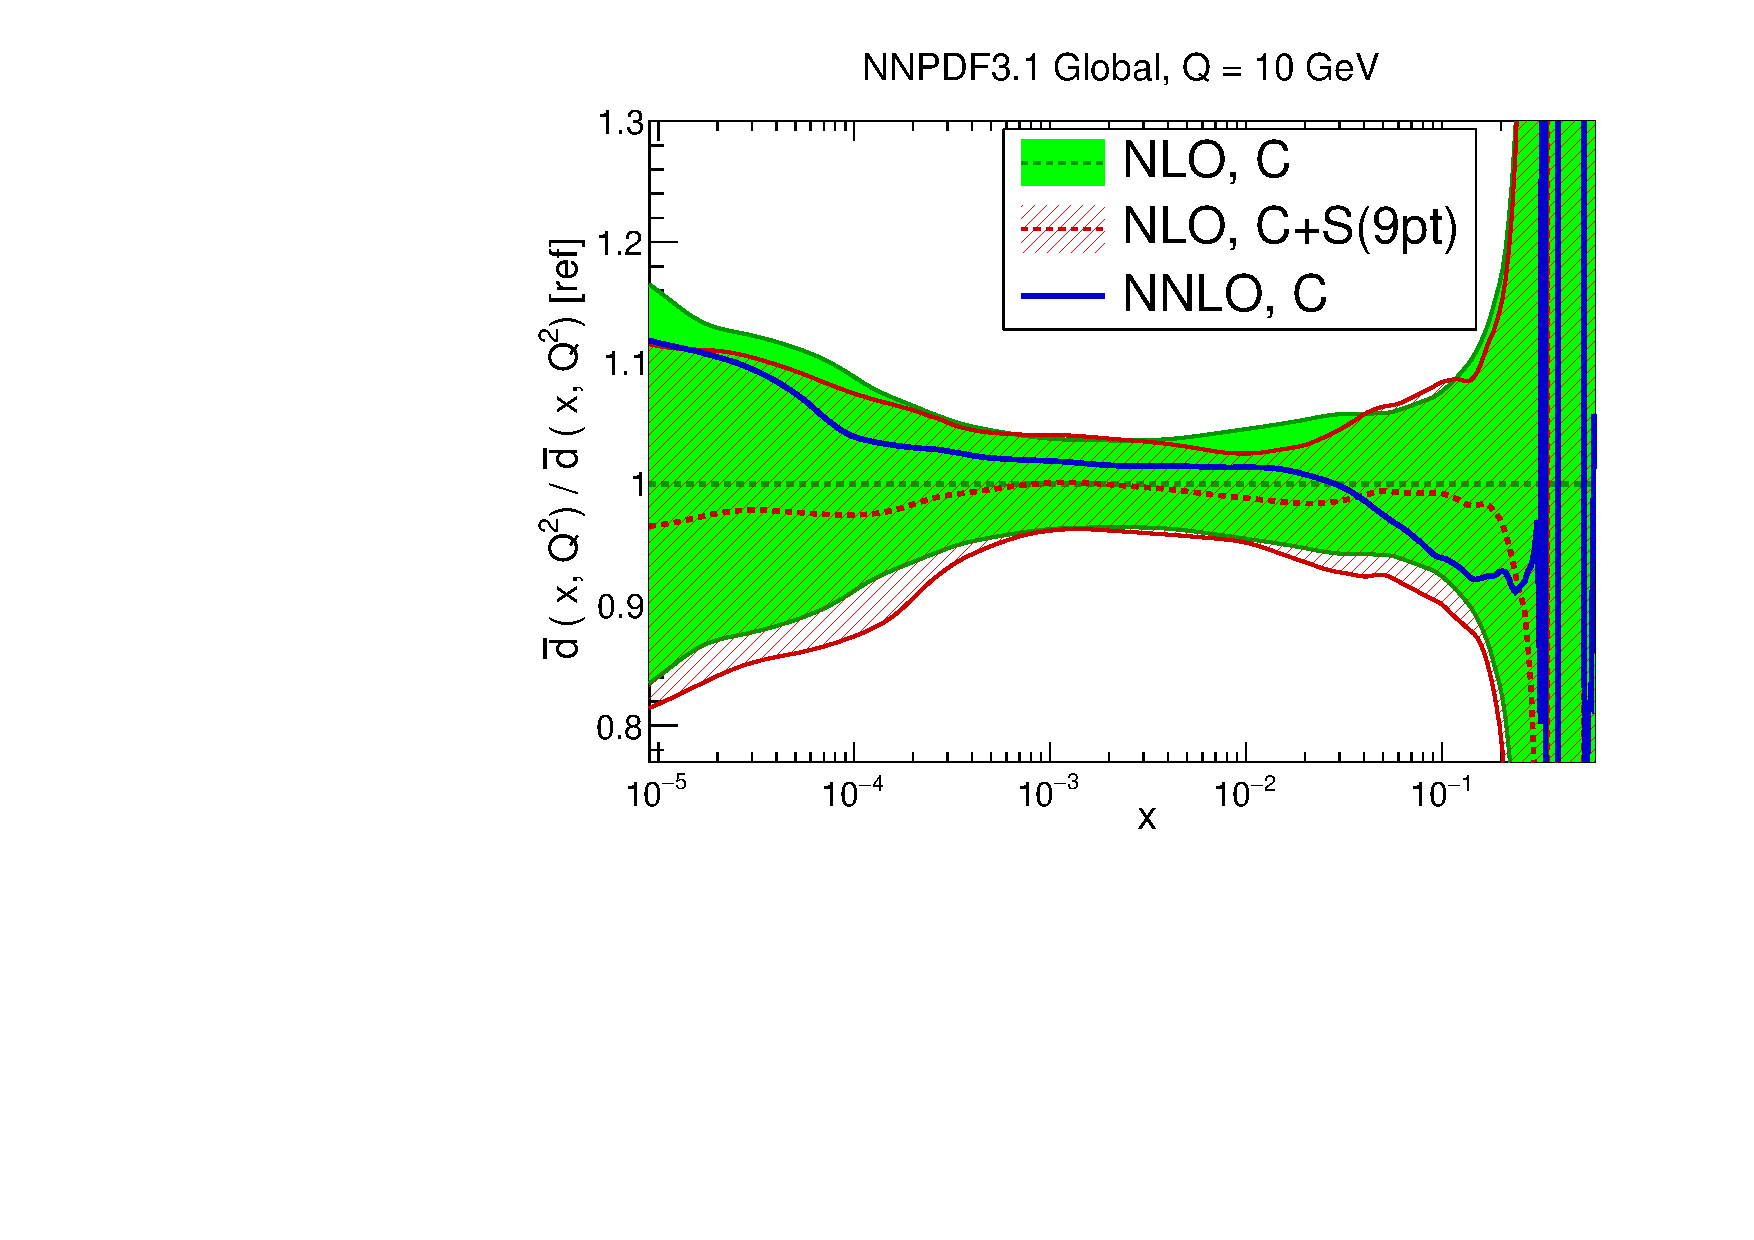
\includegraphics[width=0.49\hsize]{ch-mhou/xdbar-Global-NLO-CovMatTH-EXP-vsTH}
	\caption{
		\nnpdfr[3.1th+]{3.1th} \nlo sets, gluon and anti-down distributions at
		$\SI{10}{\giga\electronvolt}$, the first \pdf determination to include
		\mhou estimates in the fit.
	}
	\label{fig:pine/3.1th}
\end{figure}

\begin{figure}
	\centering
	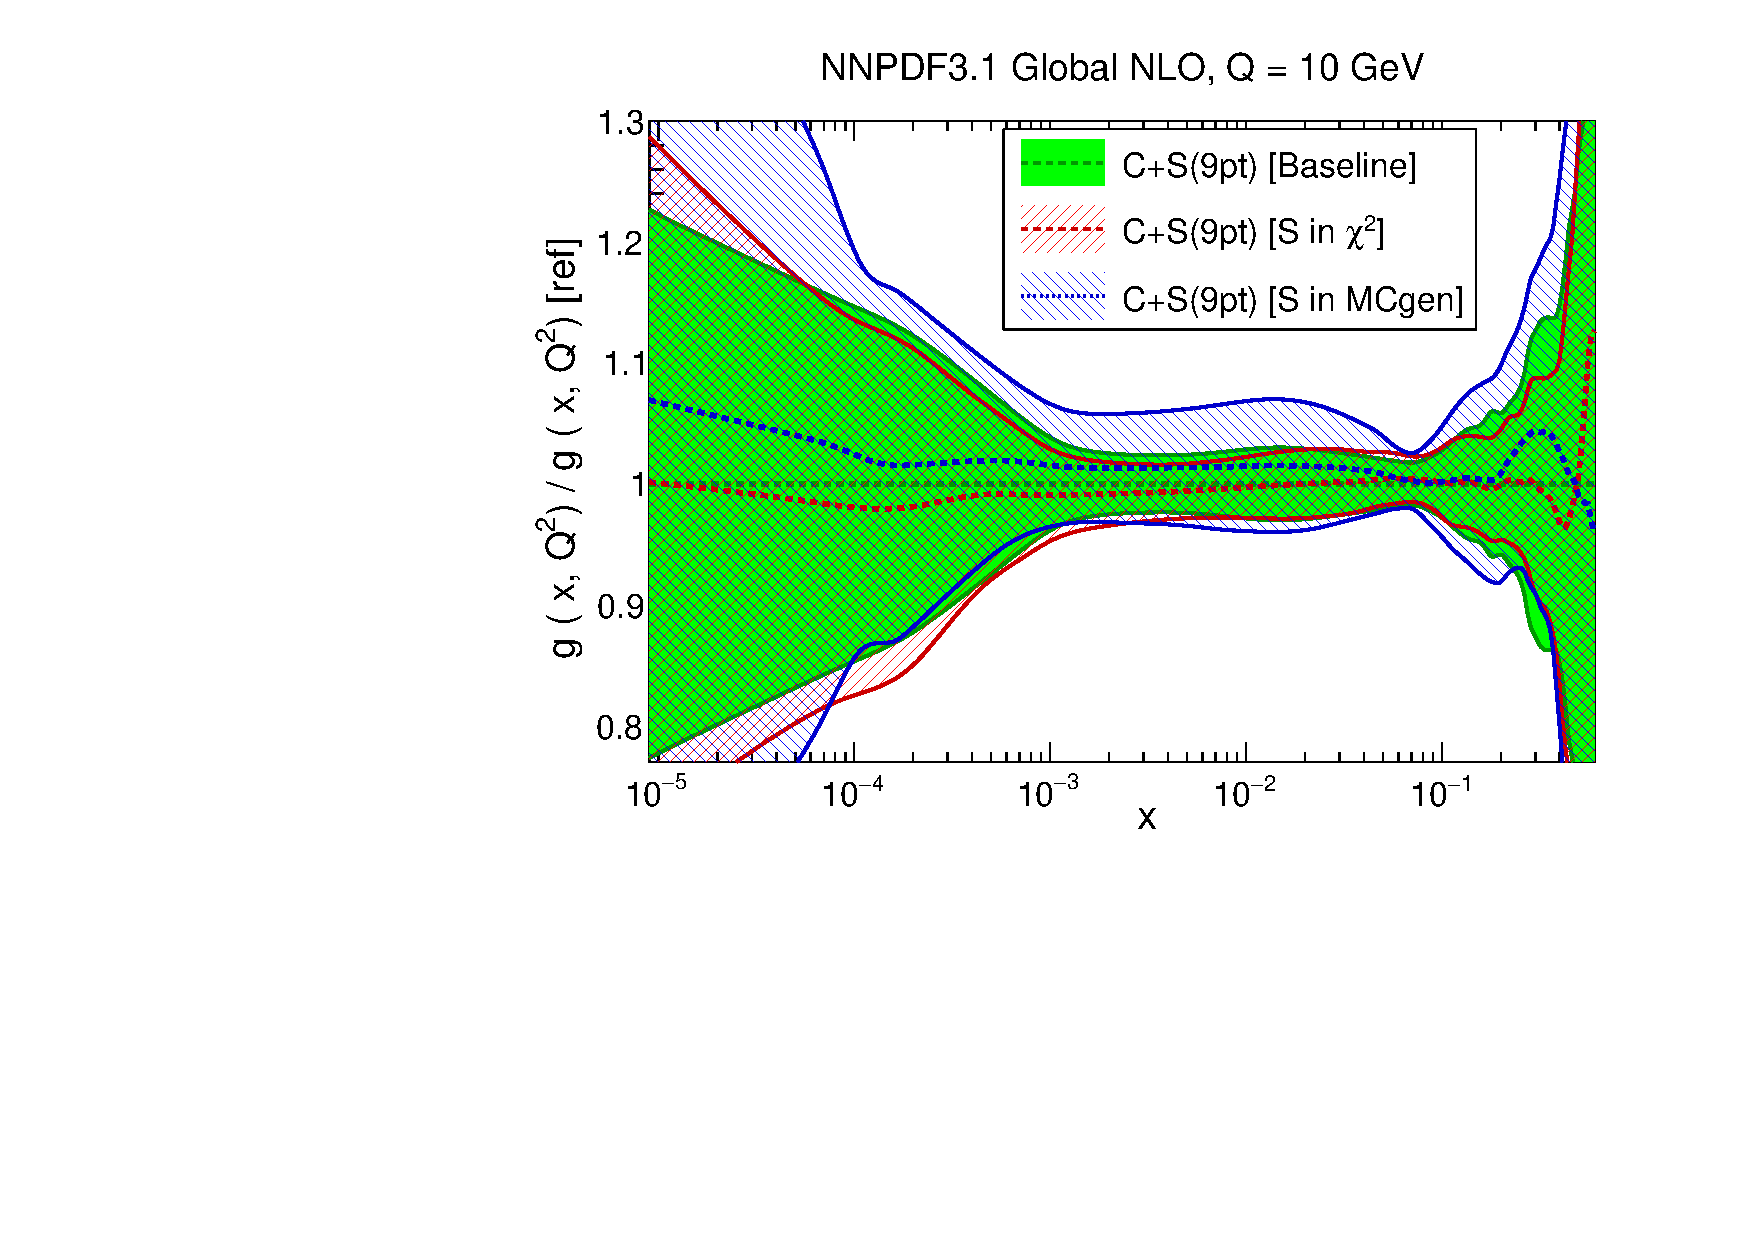
\includegraphics[width=0.49\hsize]{ch-mhou/xg-Global-NLO-CovMatTH-tests}
	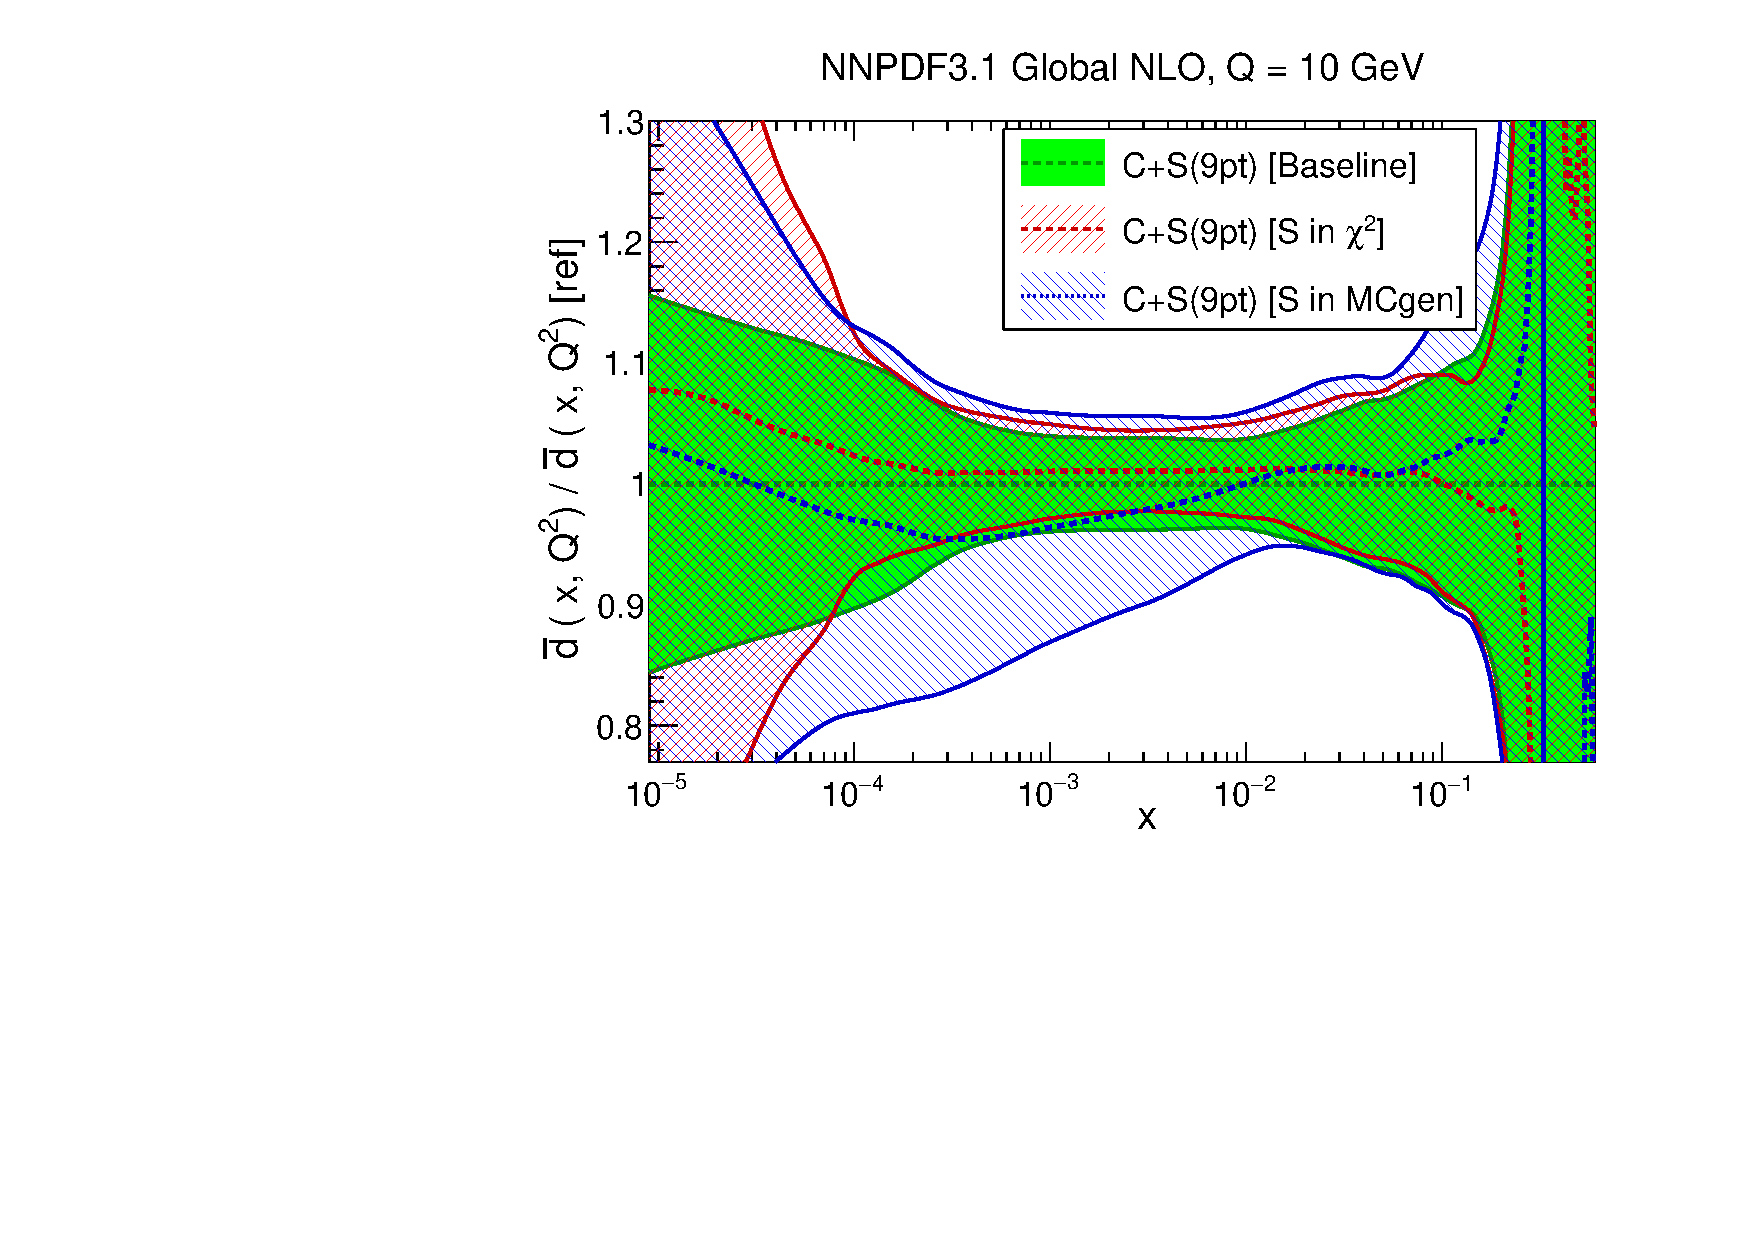
\includegraphics[width=0.49\hsize]{ch-mhou/xdbar-Global-NLO-CovMatTH-tests}
	\caption{
		Gluon and anti-down distributions comparison, in which it is shown the
		effect of using the theory covariance matrix in the $\chi^2$ or in the
		pseudo-data generation only.
	}
	\label{fig:pine/3.1th-tests}
\end{figure}
